\documentclass[12pt,letterpaper]{article} % script-article class - I like this better than article
\usepackage[margin=0.75in]{geometry}
\usepackage{graphicx}% Include figure files
\usepackage{dcolumn}% Align table columns on decimal point
\usepackage{bm}% bold math

\usepackage{helvet}
\usepackage{tikz}
\usepackage{tikz-3dplot}
\usepackage{mathtools}
\usepackage{amssymb,amsmath}
\usepackage{booktabs} % for much better looking tables
\usepackage{array} % for better arrays \left(eg matrices\right) in math
\usepackage{paralist} % very flexible & customisable lists \left(eg. enumerate/itemize, etc.\right)
\usepackage{verbatim} % adds environment for commenting out blocks of text & for better verbatim
%\usepackage[titles,subfigure]{tocloft} % Alter the style of the Table of Contents
%\usepackage{caption}
\usepackage{fixltx2e}% this might give you a warning; ignore it
%\usepackage{dblfloatfix}
\usepackage{subfig}
\usepackage{bbm}
\usepackage[space]{grffile}
\usepackage[section]{placeins}
\usepackage[justification=justified,singlelinecheck=false]{caption}
\usepackage{pdflscape}
\captionsetup[figure]{labelformat=empty}
\usepackage{tikz}
\usetikzlibrary{shapes,arrows}
\usepackage{geometry}
\usepackage{graphicx}
\usetikzlibrary{calc}
\pagenumbering{gobble}
\usepackage{array}
\usepackage{adjustbox}
\usetikzlibrary{positioning,fit}
\geometry{letterpaper,margin=0.5in}
\newcommand\addvmargin[1]{
  \node[fit=(current bounding box),inner ysep=#1,inner xsep=0]{};
}


\newcommand{\bs}[1]{\bm{\mathrm{#1}}} % always use this custom command when you want to use boldface font in a math (equation, $__$ etc.) environment.
\newcommand{\switch}[0]{\mathbbm{1}\{y_k=k\}}
\renewcommand{\epsilon}{\varepsilon}
\newcommand{\sumj}{\sum_j}

% the following are custom commands for quickly writing derivatives and partial derivatives
\newcommand{\ddt}[1]{\ensuremath{\dfrac{d#1}{dt}}}
\newcommand{\ddx}[1]{\ensuremath{\dfrac{d#1}{dx}}}
\newcommand{\ddy}[1]{\ensuremath{\dfrac{d#1}{dy}}}
\newcommand{\ddz}[1]{\ensuremath{\dfrac{d#1}{dz}}}

\newcommand{\pardt}[1]{\ensuremath{\dfrac{\partial#1}{\partial t}}}
\newcommand{\pardx}[1]{\ensuremath{\dfrac{\partial#1}{\partial x}}}
\newcommand{\pardy}[1]{\ensuremath{\dfrac{\partial#1}{\partial y}}}
\newcommand{\pardz}[1]{\ensuremath{\dfrac{\partial#1}{\partial z}}}

\newcommand{\pardtsq}[1]{\ensuremath{\dfrac{\partial^2#1}{\partial t^2}}}
\newcommand{\pardxsq}[1]{\ensuremath{\dfrac{\partial^2#1}{\partial x^2}}}
\newcommand{\pardysq}[1]{\ensuremath{\dfrac{\partial^2#1}{\partial y^2}}}
\newcommand{\pardzsq}[1]{\ensuremath{\dfrac{\partial^2#1}{\partial z^2}}}

\newcommand{\curl}[1]{\ensuremath{\nabla\times\bs{#1}}}

\newcommand{\figref}[1]{Fig.~\ref{#1}}
\newcommand{\tabref}[1]{Table~\ref{#1}}
\newcommand{\secref}[1]{Section~\ref{#1}}

%opening

\title{\Large Programming assignment 4}
\author{\large Adriana Salcedo}
\date{\large \today}

\begin{document}
\maketitle
\section{}
\subsection{}

1.Let $L{out}$ be the length of the output dimension (hieght or width), $L_{in}$ the length of the input dimenstion, $K$ as kernel size, $P$ as padding, $S$ as stride. 
\begin{align*}
\text{From the pytorch documentation:} \\
L_{out} = \frac{L_{in}-dialation(K -1) + 2P -1}{S} + 1\\
\frac{L_{in}}{2} = \frac{L_{in} - (5-1)+2P -1}{2} +1\\
L_{in} -2 = L_{in}-5-2P\\
\frac{5-2}{2} =P\\
\frac{3}{2}=P
\end{align*}
In the last layer we reduce size by a facor of four:
\begin{align*}
% \text{From the pytorch documentation:} \\
L_{out} = \frac{L_{in}-dialation(K -1) + 2P -1}{S} + 1\\
\frac{L_{in}}{4} = \frac{L_{in} - (5-1)+2P -1}{2} +1\\
\frac{L_{in}}{2} -2 = L_{in}-5-2P\\
\frac{3}{2}-\frac{L_{in}}{4} = P\\
\text{If $L_{in}$ = 4}
\frac{1}{2}=P
\end{align*}
Since a 5x5 kernel will not move across a 32x32 image symmetrically, these fractions can be approximated by rounding padding up to the nearest integer so P=2 for a two-fold reduction and P=1 for a four-fold size reduction.

\section{}

\begin{figure}[ht!]
 \subfloat[][Iteration 200 Windows emojis]
 [{
  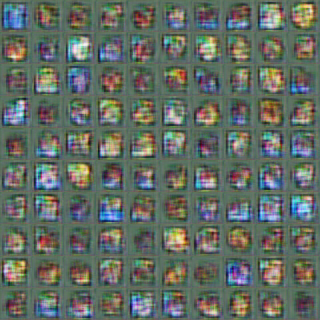
\includegraphics[width=0.4\textwidth]{dcgan_w-000200.png}
  } 
\subfloat[][Iteration 5000 Windows emojis]
 {
  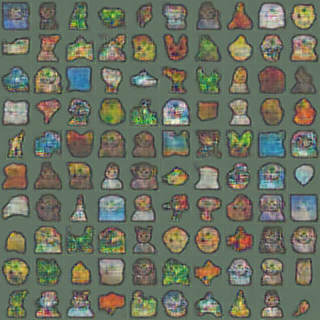
\includegraphics[width=0.4\textwidth]{dcgan_w-005000.png}
  } \hfill
\subfloat[][Iteration 1400 Apple emojis]
 {
  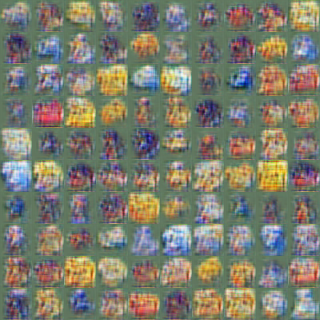
\includegraphics[width=0.4\textwidth]{dcgan-001400.png}
  } 
\subfloat[][Iteration 5000 Apple emojis]
 {
  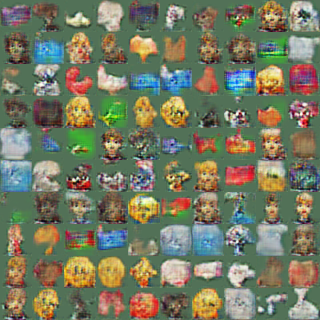
\includegraphics[width=0.4\textwidth]{dcgan-004800.png}
  } \hfill
\end{figure}
For both Windows and Apple emojis sample detail improves during training. Both begin by learning that the emojis occupy the central region of each image and some of the colours often seen in emojis, and later learn boundaries and detail.The DC-GAN is able to learn very high quality Windows emojis after 5000 iterations with clear outlines which often include a high level of detail. It 
learns lower quality Apple emojis which are less well defined and have less clear detail. This is likely because Apple emojis are more detailed and thus harder to learn so they are learned more slowly. Both learn people the best, likely because they are common in the training sets. 
\section{} 
\subsection{}
\begin{figure}[ht!]
 \subfloat[][Iteration 200 X to Y]
 {
  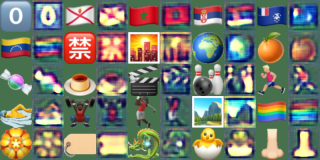
\includegraphics[width=0.4\textwidth]{cgan-000200-X-Y.png}
  } 
\subfloat[][Iteration 10000 X to Y]
 {
  
\includegraphics[width=0.4\textwidth]{cgan-010000-X-Y.png}
  } \hfill
  \subfloat[][Iteration 200 Y to X]
  {
   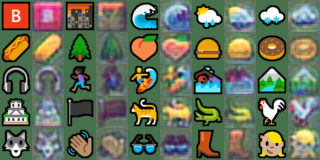
\includegraphics[width=0.4\textwidth]{cgan-000200-Y-X.png}
   } 
  \subfloat[][Iteration 10000 Y to X]
 {
  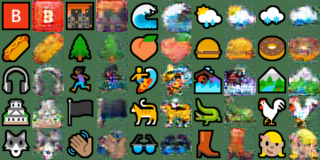
\includegraphics[width=0.4\textwidth]{cgan-010000-Y-X.png}
  } \hfill
\end{figure}
\subsection{}
\begin{figure}[ht!]
 \subfloat[][Iteration 200 X to Y]
 {
  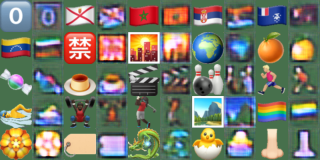
\includegraphics[width=0.4\textwidth]{cgan2-000200-X-Y.png}
  } 
\subfloat[][Iteration 10000 X to Y]
 {
  
\includegraphics[width=0.4\textwidth]{cgan2-010000-X-Y.png}
  } \hfill
  \subfloat[][Iteration 200 Y to X]
  {
   
\includegraphics[width=0.4\textwidth]{cgan2-000200-Y-X.png}
   } 
  \subfloat[][Iteration 10000 Y to X]
 {
  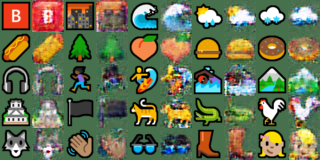
\includegraphics[width=0.4\textwidth]{cgan2-010000-Y-X.png}
  } \hfill
\end{figure}

\end{document}

